\section{Auswertung}
\subsection{Vorverstärkte Pulse auf dem Oszilloskop}
\label{VPO}
Die Pulse des Surface-Barrier Detektors werden vorverstärkt und einmal mit und einmal ohne Amplifier auf dem Oszilloskop dargestellt.
In den Abbildungen \ref{fig:2} und \ref{fig:1} werden die Pulse gegen die Zeit aufgetragen.

\begin{figure}[H]
  \centering
  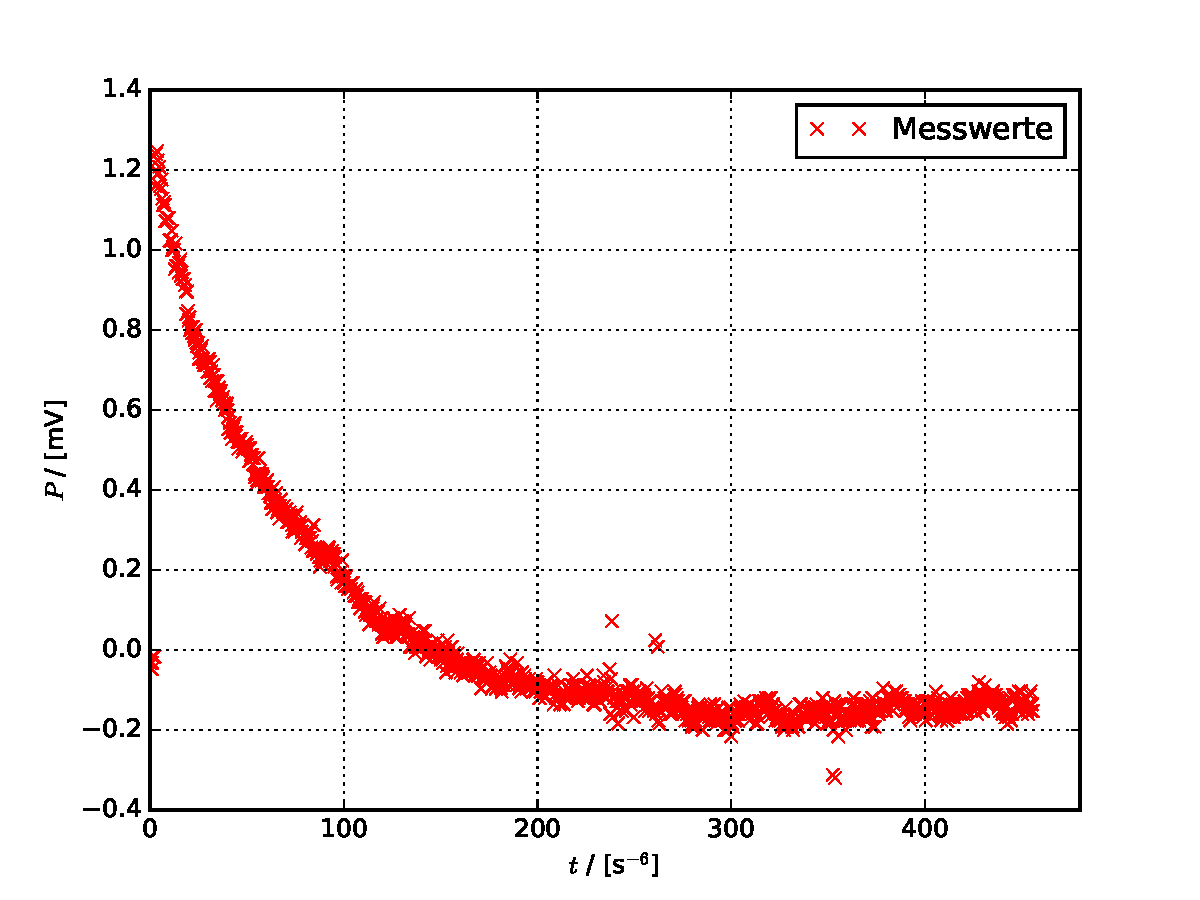
\includegraphics[width=\textwidth]{osz2.pdf}
  \caption{Pulse in Abhängigkeit von der Zeit ohne angeschlossenem Amplifier.}
  \label{fig:2}
\end{figure}

Ohne angeschlosseem Amplifier schwankt der Wert vor dem Puls um $0\,\text{V}$.
Danach steigt der Puls mit einer Anstiegszeit von $0\,\si{\micro\second}$ auf ca. $1,25\,\text{mV}$.
Mit einem "Überschwinger" pendelt sich der Wert wieder auf ca. $0\,\text{V}$ ein.

\begin{figure}[H]
  \centering
  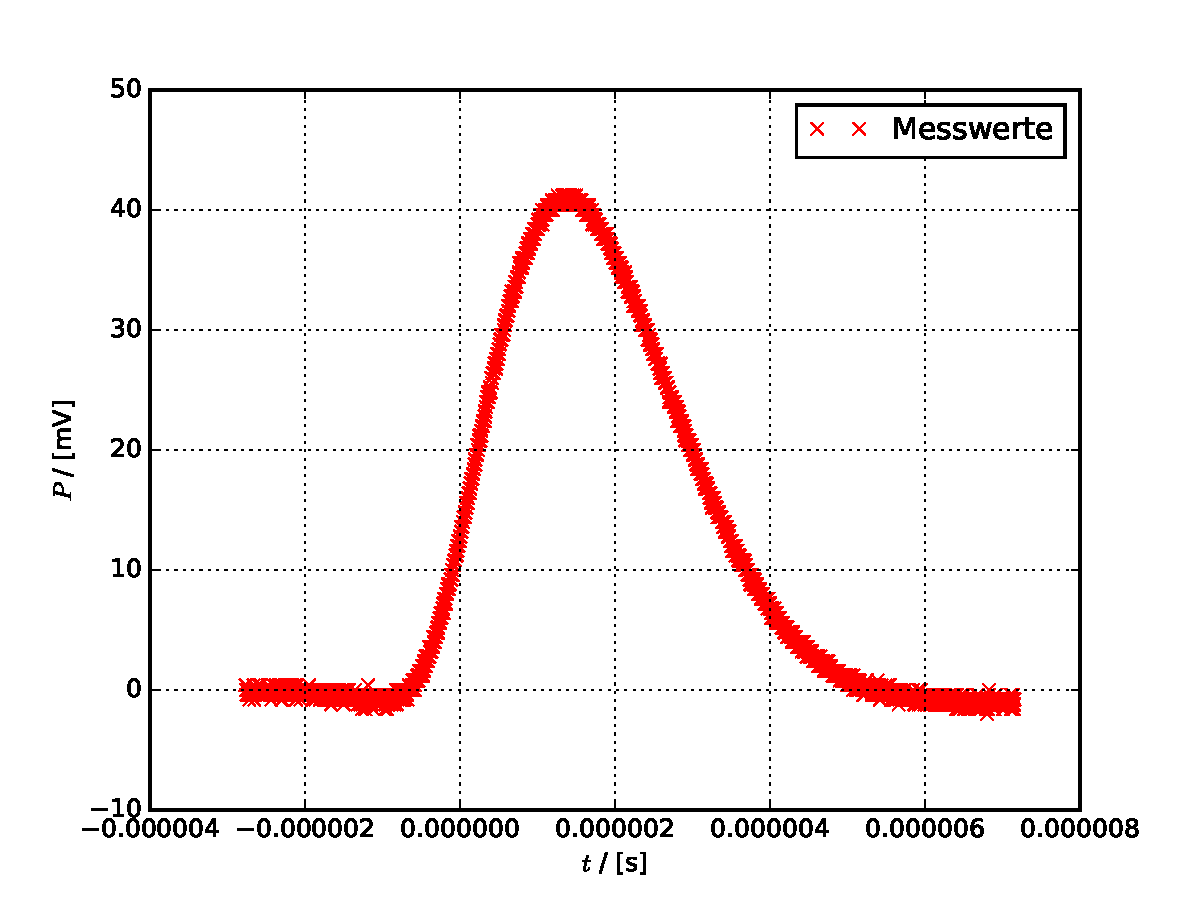
\includegraphics[width=\textwidth]{osz1.pdf}
  \caption{Pulse in Abhängigkeit von der Zeit mit angeschlossenem Amplifier.}
  \label{fig:1}
\end{figure}

Die Anstiegszeit mit angeschlossenem Amplifier beträgt ca. $8\,\si{\micro\second}$.
Der Puls steigt von $0\,\text{mV}$ auf ca. $41\,\text{mV}$ und fällt wieder auf seinen Ursprungswert ab.

\subsection{Bestimmung der Goldfoliendicke}
\label{gofodi}

In Tabelle \ref{tab:U(p)} sind die Messwerte für die Pulshöhen des Detektors in Abhängigkeit vom Kammerdruck zu entnehmen.

\begin{table}[H]
  \centering
  \begin{tabular}{cc|cc}
    \toprule
    \multicolumn{2}{c}{Mit Goldfolie} & \multicolumn{2}{c}{Ohne Goldfolie} \\
    Pulshöhe [V] & Druck [mbar] & Pulshöhe [V] & Druck [mbar] \\
    \midrule
    1.020 & 0.025 & 1.310 & 0.075 \\
    0.936 & 0.639 & 1.260 & 0.290 \\
    0.896 & 7.900 & 1.210 & 51.20 \\
    0.832 & 18.30 & 1.140 & 84.90 \\
    0.752 & 38.00 & 1.050 & 110.5 \\
    0.632 & 61.10 & 0.928 & 126.6 \\
    0.512 & 109.1 & 0.856 & 141.6 \\
    0.680 & 95.70 & 0.728 & 157.5 \\
    0.800 & 75.60 & 0.672 & 174.6 \\
    0.840 & 57.20 & 0.904 & 136.9 \\
    0.984 & 45.00 & 1.010 & 116.0 \\
    1.000 & 21.50 & 1.120 & 93.30 \\
    1.090 & 1.500 & 1.180 & 74.00 \\
    \bottomrule
  \end{tabular}
  \caption{Puls in Abhängigkeit vom Kammerdruck.}
  \label{tab:U(p)}
\end{table}

In Abbildung \ref{fig:U(p)} sind die Pulse in Abhängigkeit vom Kammerdruck aufgetragen.
Außerdem wird eine Ausgleichsrechnung der Form $y=ax+b$ durchgeführt.

\begin{figure}[H]
  \centering
  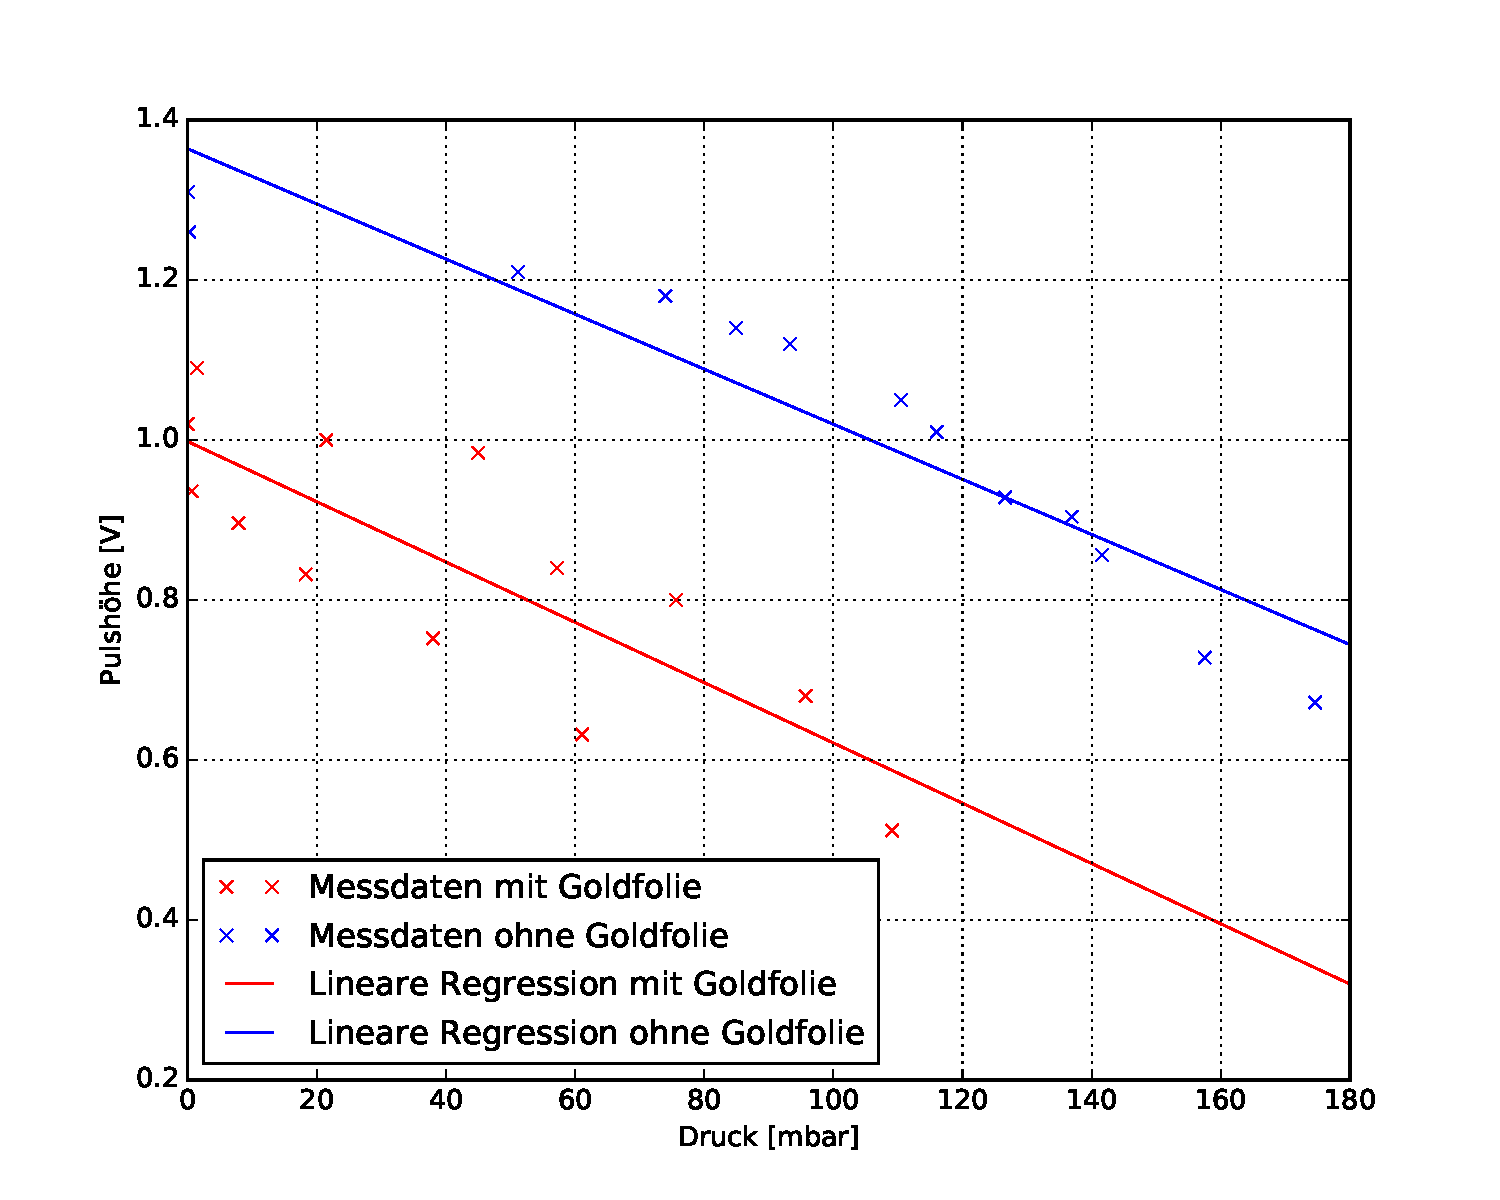
\includegraphics[width=\textwidth]{pulshohe_druck2.pdf}
  \caption{Pulse in Abhängigkeit vom Druck mit und ohne Goldfolie und lineare Regression beider Messreihen.}
  \label{fig:U(p)}
\end{figure}

Für die Parameter folgt
\begin{gather*}
  \textcolor{red}{a_1 = (-0,0038 \pm 0,0008)\,\frac{\text{V}}{\text{mbar}}}, \\
  \textcolor{red}{b_1 = (1,00 \pm 0,04)\,\text{V}}, \\
  \textcolor{blue}{a_2 = (0,0034 \pm 0,0004)\,\frac{\text{V}}{\text{mbar}}}, \\
  \textcolor{blue}{b_2 = (1,36 \pm 0,04)\,\text{V}}.
\end{gather*}
Der $y$-Achsenabschnitt $b_2$ der Messreihe ohne Goldfolie gibt an,
wie hoch die Energie eines Alphateilchens im Vakuum ist.
Der Abbildung \ref{fig:amnp} kann entnommen werden,
dass die mittlere kinetische Energie des $\alpha$-Teilchens $E_{\alpha} = 5,48\,\text{MeV}$ beträgt.
Somit entspricht die Pulshöhe der mittleren kinetischen Energie des $\alpha$-Teilchens:
\begin{align}
  b_2 = 1,36 \propto E_{\alpha} = 5,48\,\text{MeV}.
  \label{eqn:bE}
\end{align}
Mit diesem Wissen kann der Energieverlust berechnet werden.
Der Pulsverlust ist gegeben durch
\begin{equation}
  \Delta{P} = b_2-b_1.
\end{equation}
Der Fehler beträgt unter Berücksichtigung der Gaußschen Fehlerfortpflanzung
\begin{equation}
  \Delta(\Delta{P}) = \sqrt{(\Delta{b_2})^2 + (\Delta{b_1})^2}.
\end{equation}
Somit ist ergibt sich
\begin{align*}
  \Delta{P}\pm\Delta(\Delta{P}) = (0,36\pm0,06)\,\text{V}
\end{align*}
Durch den proportionalen Zusammenhang \eqref{eqn:bE} ergibt sich aus dem Pulsverlust der Energieverlust
\begin{align*}
  \Delta{E} = \frac{E_{\alpha}}{b_2}\cdot{\Delta{P}} = (1,45\pm0,25)\,\text{MeV}.
\end{align*}
Um die Dicke der Goldfolie zu bestimmen, wird die Bethe-Bloch-Gleichung \eqref{eqn:bloch} nach $dx$ umgestellt.
Für die Foliendicke ergibt sich die Formel
\begin{equation}
  \Delta{x} = -\Delta{E}\cdot\left( \ln\left( \frac{2m_0v^2}{I} \right) \right)^{-1}\cdot\left(\frac{m_0v^2(4\pi\epsilon_0)^2}{4\pi\text{e}^4z^2nZ}\right).
\end{equation}
Die Geschwindigkeit des $\alpha$-Teilchens lässt sich mit
\begin{align*}
  v = v_{\alpha} = \sqrt{ \frac{2\cdot{E_{\alpha}}}{m_{\alpha}} } = 1,625\cdot10^{7}\,\frac{\text{m}}{\text{s}}
\end{align*}
berechnen, wobei $m_{\alpha} = 4\,\text{u}$ \cite{chem} die Masse des $\alpha$-Teilchens ist.
Die Ionisationsenergie von Gold beträgt $I_{\text{Au}} = 9,225\,\text{eV}$ \cite{PSE}.
Die Ladungzahl des $\alpha$-Teilchens ist $z = 2$, wobei $e$ die Elementarladung ist.
Die Kernladungszahl von Gold ist $Z = 79$ \cite{PSE}.
Die Teilchendichte lässt sich mit
\begin{align*}
  n = \frac{\rho_{\text{Au}}}{m_{\text{Au}}}
\end{align*}
berechnen.
Die Dichte von Gold beträgt $\rho_{\text{Au}} = 19,302\,\frac{\text{g}}{\text{cm}^3}$ \cite{PSE} und die Masse $m_{\text{Au}} = 196,967\,\text{u}$ \cite{PSE}.
Es ergibt sich eine Foliendicke von
\begin{equation*}
  \Delta{x} = (1,55\pm0,27)\cdot10^{-6}\,\text{m}.
\end{equation*}

\subsection{Bestimmung des differentiellen Wirkungsquerschnitts}
\label{kap:WQ}
In Tabelle \ref{tab:WQ} sind die Messwerte zur Bestimmung des differentiellen Wirkungsquerschnittes zu entnehmen.

\begin{table}[H]
  \centering
  \begin{tabular}{ccc|ccc}
    \toprule
    Winkel & Counts & Zeit & Winkel & Counts & Zeit \\
    $\theta$ [°] & c & $t$ [s] & $\theta$ [°] & c & $t$ [s] \\
    \midrule
    0,0 &  916 & 100 &  1,9 & 1145 & 110  \\
    0,1 &  885 & 100 &  2,0 & 1209 & 110  \\
    0,2 &  942 & 100 &  2,1 & 1197 & 110  \\
    0,3 & 1058 & 100 &  2,2 & 1127 & 110  \\
    0,4 &  959 & 100 &  2,3 & 1142 & 110  \\
    0,5 & 1067 & 100 &  2,4 & 1100 & 110  \\
    0,6 & 1185 & 110 &  2,5 & 1164 & 110  \\
    0,7 & 1071 & 110 &  2,6 & 1164 & 110  \\
    0,8 & 1139 & 110 &  2,7 & 1223 & 110  \\
    0,9 & 1160 & 110 &  2,8 & 1103 & 110  \\
    1,0 & 1093 & 110 &  2,9 & 1232 & 110  \\
    1,1 & 1230 & 110 &  3,0 & 1107 & 110  \\
    1,2 & 1164 & 110 &  4,0 & 1092 & 110  \\
    1,3 & 1133 & 110 &  6,0 &  872 & 120  \\
    1,4 & 1143 & 110 &  8,0 & 1140 & 300  \\
    1,5 & 1157 & 110 & 10,0 &  994 & 450  \\
    1,6 & 1215 & 110 & 15,0 &  851 & 1200 \\
    1,7 & 1183 & 110 & 20,0 &  543 & 900  \\
    1,8 & 1165 & 110 &                    \\
    \bottomrule
  \end{tabular}
  \caption{Messwerte der Counts pro Zeit in Abhängigkeit vom Detektorwinkel.}
  \label{tab:WQ}
\end{table}
Die Rate $\sfrac{c}{t}$ der Counts pro Zeit werden durch Division der Counts durch die gemessene Zeit erhalten.
Der Fehler der Rate ist gegeben durch
\begin{equation}
  \Delta{\frac{c}{t}} = \sqrt{\frac{c}{t}},
\end{equation}
da der $\alpha$-Zerfall der Poissonverteilung unterliegt.
Der empirische differentielle Wirkungsquerschnitt kann durch
\begin{equation}
  \frac{d\sigma}{d\Omega}(\theta) = \frac{c/t}{A\cdot{N}\cdot\Delta{x}\cdot d\Omega^2}
  \label{WQbla}
\end{equation}
berechnet werden.
Dabei ist $A = (15,75\pm3,98)\,\text{Bq}$ die Aktivität der verwendeten Americium-Quelle, $N = 5,9\cdot10^{28}\,\text{m}^{-3}$ die Anzahl der Streuzentren,
$\Delta{x} = 2\,\si{\micro\metre}$ die Foliendicke und $\Omega$ der Raumwinkel.
Der Raumwinkel ist gegeben durch
\begin{equation}
  \Omega = 4\arctan\left( \frac{x}{2l} \right)\arctan\left( \frac{y}{2l} \right) = 9,8\cdot10^{-3},
\end{equation}
wobei $x = 2\,\text{mm}$ und $y=10\,\text{mm}$ die Seitenlängen der bestrahlten Blende und
$l = 4,5\,\text{cm}$ der Abstand der Goldfolie zum Detektor sind.
Der Fehler nach Gauß des differentiellen Wirkungsquerschnittes ist gegeben durch
\begin{equation}
  \Delta{\frac{d\sigma}{d\Omega}} = \sqrt{ \left(\frac{\Delta(c/t)}{A\cdot{N}\cdot\Delta{x}\cdot d\Omega^2}\right)^2 + \left( -\frac{(c/t)\cdot\Delta{A}}{A^2\cdot{N}\cdot\Delta{x}\cdot d\Omega^2} \right) }.
\end{equation}

Der theoretische Wirkungsquerschnitt lässt sich mittels der Formel \eqref{eqn:streu} berechnen.
In Tabelle \ref{tab:WQ} sind die berechneten Wirkungsquerschnitte zu den Winkeln aufgelistet.
Der zugehörige Plot ist in Abbildung \ref{fig:WQ} einzusehen.
Die theoretischen Wirkungsquerschnitte bis einschließlich dem Winkel $\theta = 1,2°$ wurden übersichtshalber herausgenommen.

\begin{figure}[H]
  \centering
  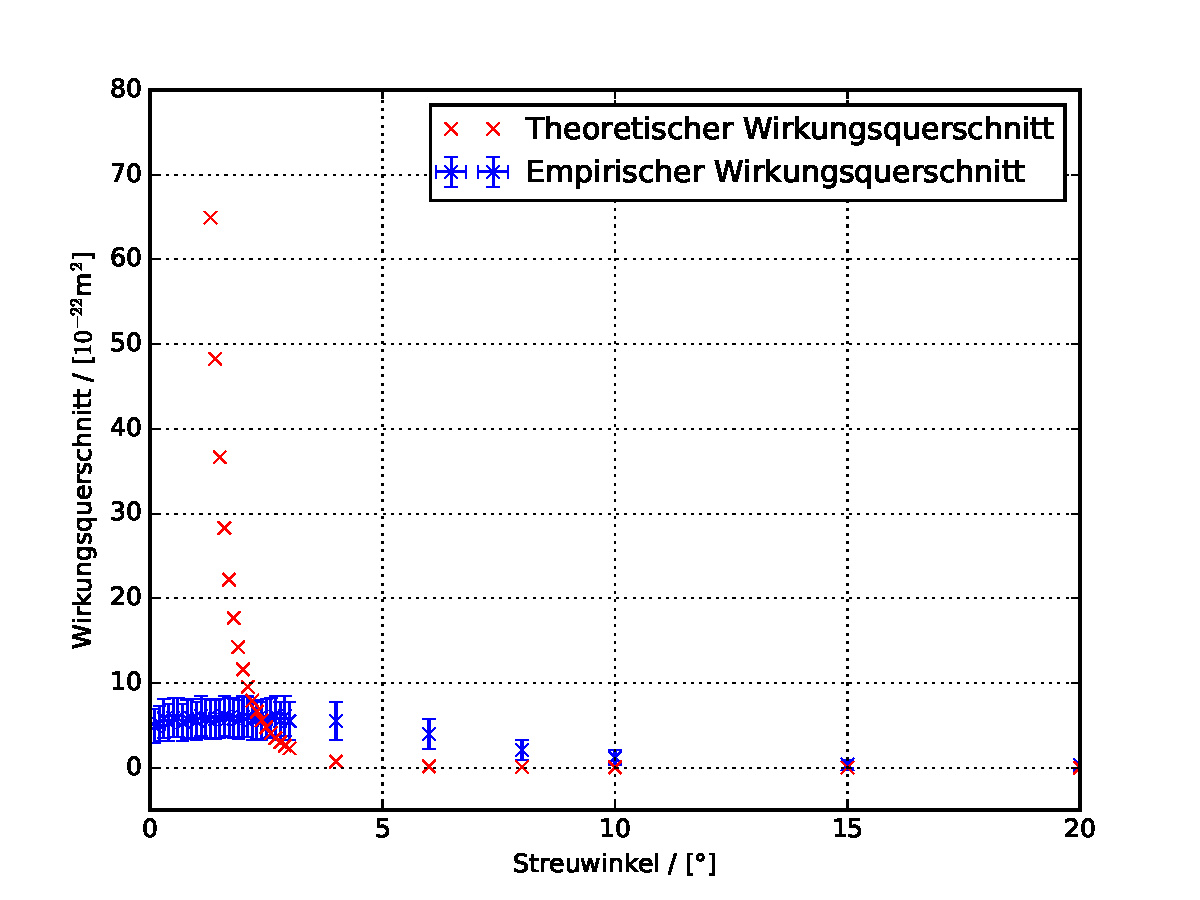
\includegraphics[width=\textwidth]{WQ.pdf}
  \caption{Theoretischer und empirischer Wirkungsquerschnitt in Abhängigkeit vom Winkel.}
  \label{fig:WQ}
\end{figure}
\begin{table}
[H]
  \center
\begin{tabular}{c|c|c}
\toprule

Winkel & \multicolumn{2}{c}{Wirkungsquerschnitt} \\
       &
 theoretisch & empirisch \\
$\theta$ [°]
& $\frac{d\sigma}{d\Omega}_{\text{theo}}$ [$10^{-22}\frac{1}{\text{m}}$]
& $\frac{d\sigma}{d\Omega}_{\text{emp}}$ [$10^{-22}\frac{1}{\text{m}}$] \\
\midrule
 0.1 & 1854289,3 & $(4,9\pm2,0)$\\

 0.2 & 115893,26 & $(5,2\pm2,1)$\\

 0.3 & 22892,554 & $(5,8\pm2,3)$\\

 0.4 & 7243,3729 & $(5,3\pm2,2)$\\

 0.5 & 2966,8991 & $(5,9\pm2,3)$\\

 0.6 & 1430,8042 & $(5,9\pm2,3)$\\

 0.7 & 772,31759 & $(5,3\pm2,2)$\\

 0.8 & 452,72183 & $(5,7\pm2,3)$\\

 0.9 & 282,63445 & $(5,8\pm2,3)$\\

 1.0 & 185,43825 & $(5,5\pm2,2)$\\

 1.1 & 126,65817 & $(6,1\pm2,4)$\\

 1.2 & 89,430168 & $(5,8\pm2,3)$\\

 1.3 & 64,929362 & $(5,7\pm2,3)$\\

 1.4 & 48,273451 & $(5,7\pm2,3)$\\

 1.5 & 36,632103 & $(5,8\pm2,3)$\\

 1.6 & 28,297873 & $(6,1\pm2,4)$\\

 1.7 & 22,204720 & $(5,9\pm2,3)$\\

 1.8 & 17,666832 & $(5,8\pm2,3)$\\

 1.9 & 14,231231 & $(5,7\pm2,3)$\\

 2.0 & 11,591656 & $(6,0\pm2,4)$\\

 2.1 & 9,5366828 & $(6,0\pm2,4)$\\

 2.2 & 7,9175948 & $(5,6\pm2,3)$\\

 2.3 & 6,6280012 & $(5,7\pm2,3)$\\

 2.4 & 5,5906115 & $(5,5\pm2,2)$\\

 2.5 & 4,7484848 & $(5,8\pm2,3)$\\

 2.6 & 4,0591298 & $(5,9\pm2,3)$\\

 2.7 & 3,4904624 & $(6,1\pm2,4)$\\

 2.8 & 3,0179915 & $(5,5\pm2,2)$\\

 2.9 & 2,6228335 & $(6,1\pm2,4)$\\

 3.0 & 2,2902912 & $(5,5\pm2,2)$\\

 4.0 & 0,7249200 & $(5,5\pm2,2)$\\

 6.0 & 0,1433395 & $(4,0\pm1,8)$\\

 8.0 & 0,0454180 & $(2,1\pm1,2)$\\

10.0 & 0,0186372 & $(1,2\pm0,9)$\\

15.0 & 0,0037048 & $(0,4\pm0,5)$\\

20.0 & 0,0011827 & $(0,3\pm0,4)$\\

\bottomrule
\end{tabular}

\caption{Theoretische und empirische Wirkungsquerschnitte in Abhängigkeit von den Winkeln.}
\label{tab:WQ}
\end{table}



\subsection{Untersuchung des Einflusses der Mehrfachstreuung}
\label{kap:mfs}
In folgender Tabelle \ref{tab:mfs} sind die Messwerte der Zählrate zweier verschieden dicker Goldfolien einzusehen.

\begin{table}[H]
  \centering
  \begin{tabular}{cc}
    \toprule
    Dicke [$\si{\micro\metre}$] & Zählrate $\left[\frac{1}{\text{s}}\right]$ \\
    \midrule
    2 & $(10,06\pm3,17)$\\
    4 & $(0,85\pm0,92)$\\
    \bottomrule
  \end{tabular}
  \caption{Zählrate zweier Goldfolien verschiedener Dicke.}
  \label{tab:mfs}
\end{table}

\subsection{Ordnungszahl-Abhängigkeit des Wirkungsquerschnittes}
\label{5.5}
Analog zum Abschnitt \ref{kap:WQ} wird der Wirkungsquerschnitt verschiedener Materialien bei einem festen Winkel von $\theta = 3°$ berechnet.
In Tabelle \ref{tab:Z-WQ} sind die relevanten Stoffeigenschaften der verschiedenen Teilchen und die berechneten Wirkungsquerschnitte aufgelistet.
\begin{table}[H]
  \centering
  \begin{tabular}{cccccc}
    \toprule
    Dicke & Ordnungszahl & Teilchendichte & Countrate  & Theoretischer & Empirischer \\
          &               &               &             & Wirkungsquerschnitt & Wirkungsquerschnitt \\
    $\Delta{x}$ [$\si{\micro\metre}$] & $Z$ & $N$ [$10^{28}$m$^{-3}$]
    & $R$ [s$^{-1}$] & $\frac{d\sigma}{d\Omega}_{theo}$ [$10^{-22}$m$^{2}$] & $\frac{d\sigma}{d\Omega}_{emp}$ [$10^{-22}$m$^{2}$] \\
    \midrule
    2 & 79 & 5.9 & 10.06 \pm 3.17 & 2.29 & 5.50 \pm 2.20 \\
    3 & 13 & 6.2 & 0.94  \pm 0.97 & 0.06 & 0.33 \pm 0.35 \\
    1 & 83 & 2.9 & 0.52  \pm 0.72 & 2.50 & 1.20 \pm 1.60 \\
    \bottomrule
  \end{tabular}
  \caption{Relevante Stoffeigenschaften \cite{PSE} und Wirkungsquerschnitte.}
  \label{tab:Z-WQ}
\end{table}

In Abbildung \ref{fig:Z-WQ} werden die theoretischen und empirischen Wirkungsquerschnitte aufgetragen.

\begin{figure}[H]
  \centering
  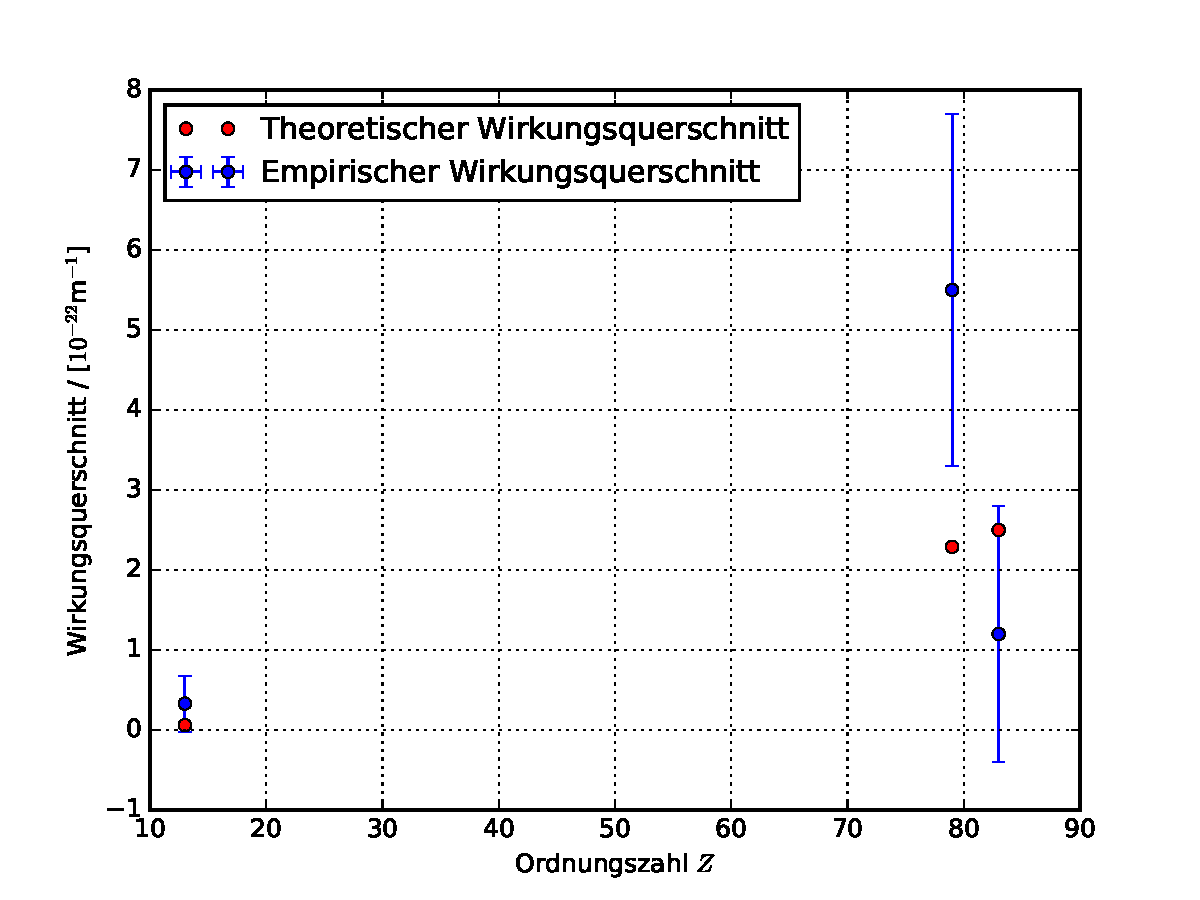
\includegraphics[width=\textwidth]{Z-WQ.pdf}
  \caption{Theoretische und empirische Wirkungsquerschnitte von Gold, Aluminium und Bismut in Abhängigkeit derer Ordnungszahl.}
  \label{fig:Z-WQ}
\end{figure}
